\section{A convolutional model of STM}
A convolutional model of STM interpret STM spectroscopy measurement as the convolution of the features sourced from defects and their corresponding activation. The first convolutional model of STM was raised by Cheung et al \cite{cheungDictionaryLearningFouriertransform2020}; As shown in Figure \ref{fig:ch6_conv} a), an STM observation Y is the convolution of a kernel $A_0$ and its corresponding activation $X_0$. we extend the convolutional model to multi-type defect case, as hinted in Figure \ref{fig:ch6_demix}, we now have multiple kernels $A_d$ with different sizes and their corresponding activation map $X_d$. This is exactly what we formulated in the demixing problem with Equation \ref{eq:demixing}:

\begin{equation}
	Y_{\omega} = \sum_d ( A_{d,{\omega}} * X_d) + \beta. 
\end{equation}

\noindent It is worth noting that the kernels could vary in different energy slices, as the energy dispersion of QPI patterns are normally non-trivial, and the noise level may also vary at different energies. On the other hand, the activation map should stay the same across all energies, as the defect location should be fixed. The task of recovering all $A_d$ and $X_d$ given $Y$ is known as the \ac{MC-SBD} problem. 
 
\begin{figure}
	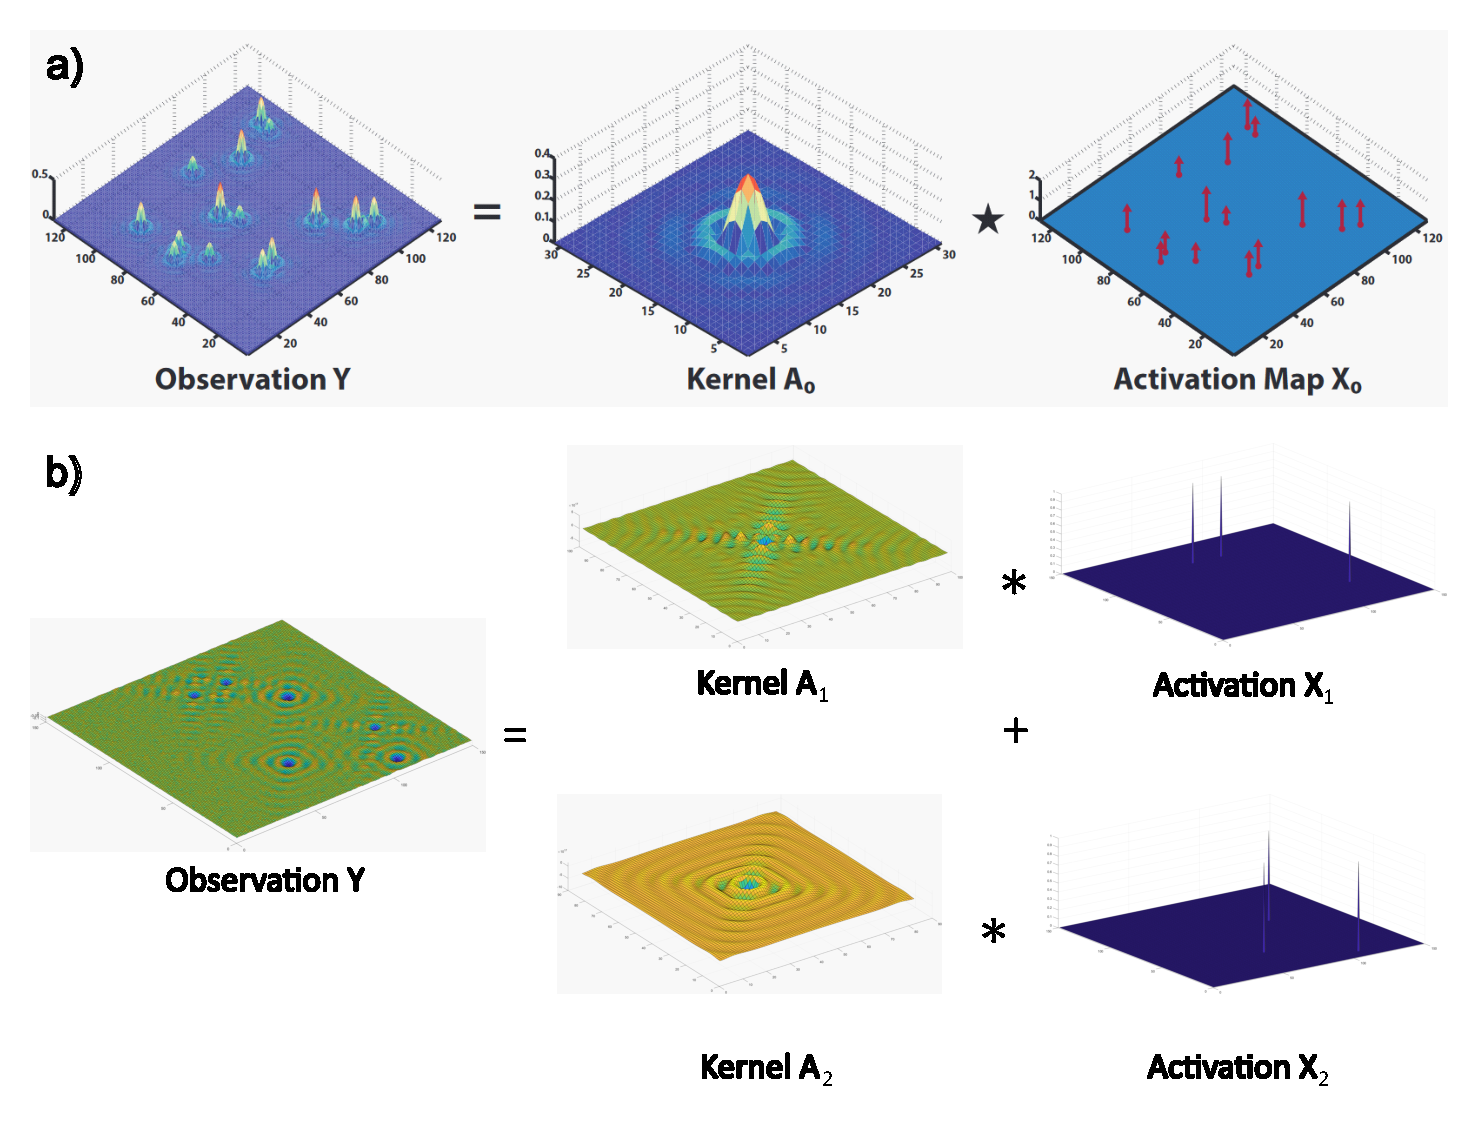
\includegraphics[width= \textwidth]{convolutional_model.pdf} 
	\centering
	\caption{Convolutional model of STM grid spectroscopy. a) Single defect convolutional model, introduced by Cheung et al to solve Sparse Blind Deconvolution(SBD) problem.\cite{cheungDictionaryLearningFouriertransform2020}. b) Multi-defect convolutional model, used to address \ac{MC-SBD} problem.}
	\label{fig:ch6_conv}
\end{figure}


\subsection{formulation of Multi-Channel Sparse Blind Deconvolution problem}

